\documentclass[tikz,border=5pt]{standalone}
\usepackage{ctex,amsmath}
\usetikzlibrary{arrows.meta,calc}
\tikzset{>=Latex,axis/.style={gray,thin,->},field/.style={orange!85!black,thick,->},event/.style={blue!65!black},guide/.style={gray,dashed}}
\begin{document}
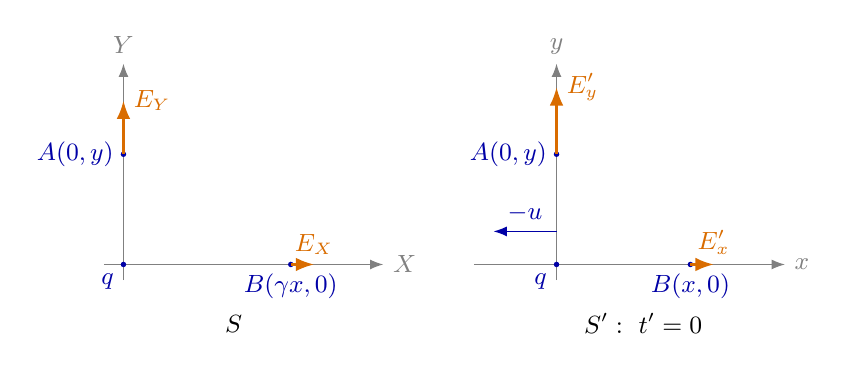
\begin{tikzpicture}[font=\small]
\begin{scope}
\draw[axis](-.25,0)--(3.3,0)node[right]{$X$};
\draw[axis](0,-.2)--(0,2.55)node[above]{$Y$};
\fill[event](0,0)circle[radius=.035]node[below left]{$q$};
\fill[event](0,1.4)circle[radius=.035]node[left]{$A(0,y)$};
\fill[event](2.125,0)circle[radius=.035]node[below]{$B(\gamma x,0)$};
\draw[field](0,1.4)--(0,2.08)node[right]{$E_Y$};
\draw[field](2.125,0)--(2.420152,0)node[above]{$E_X$};
\node at(1.4,-.75){$S$};
\end{scope}
\begin{scope}[xshift=5.5cm]
\draw[axis](-1.05,0)--(2.9,0)node[right]{$x$};
\draw[axis](0,-.2)--(0,2.55)node[above]{$y$};
\fill[event](0,0)circle[radius=.035]node[below left]{$q$};
\fill[event](0,1.4)circle[radius=.035]node[left]{$A(0,y)$};
\fill[event](1.7,0)circle[radius=.035]node[below]{$B(x,0)$};
\draw[field](0,1.4)--(0,2.25)node[right]{$E'_y$};
\draw[field](1.7,0)--(1.995152,0)node[above]{$E'_x$};
\draw[blue!65!black,->](0,.42)--(-.8,.42)node[midway,above]{$-u$};
\node at(1.1,-.75){$S':\ t'=0$};
\end{scope}
\end{tikzpicture}
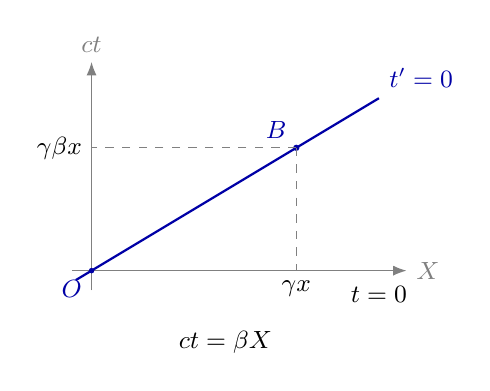
\begin{tikzpicture}[font=\small]
\draw[axis](-.25,0)--(4,0)node[right]{$X$};
\draw[axis](0,-.25)--(0,2.65)node[above]{$ct$};
\draw[blue!65!black,thick](-.2,-.12)--(3.65,2.19)node[above right]{$t'=0$};
\fill[event](0,0)circle[radius=.035]node[below left]{$O$};
\fill[event](2.6,1.56)circle[radius=.04]node[above left]{$B$};
\draw[guide](2.6,1.56)--(2.6,0)node[below,text=black]{$\gamma x$};
\draw[guide](2.6,1.56)--(0,1.56)node[left,text=black]{$\gamma\beta x$};
\node[below]at(3.65,-.08){$t=0$};
\node[below]at(1.7,-.65){$ct=\beta X$};
\end{tikzpicture}
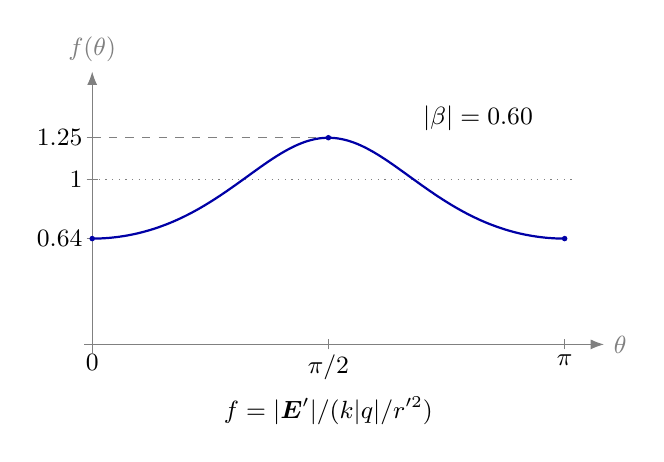
\begin{tikzpicture}[font=\small,x=1cm,y=2.1cm]
\draw[axis](-.1,0)--(6.5,0)node[right]{$\theta$};
\draw[axis](0,-.05)--(0,1.65)node[above]{$f(\theta)$};
\draw[gray,dotted](0,1)--(6.1,1);
\draw[guide](0,1.25)--(3,1.25);
\foreach \yy in {0.64,1,1.25}{\draw[gray](-.07,\yy)--(.07,\yy)node[left,xshift=-2pt,text=black]{$\yy$};}
\foreach \xx/\lab in {0/0,3/{\pi/2},6/\pi}{\draw[gray](\xx,-.03)--(\xx,.03)node[below,yshift=-2pt,text=black]{$\lab$};}
\draw[blue!65!black,thick,domain=0:180,samples=161]plot({\x/30},{.64/(1-.36*sin(\x)^2)^1.5});
\foreach \pt in {(0,.64),(3,1.25),(6,.64)}\fill[blue!65!black]\pt circle[radius=.035cm];
\node at(4.9,1.37){$|\beta|=0.60$};
\node[below]at(3,-.26){$f=|\boldsymbol E'|/(k|q|/r'^2)$};
\end{tikzpicture}
\end{document}
